\documentclass[a4paper,12pt]{article}

\usepackage[utf8]{inputenc}
\usepackage{amsmath, amssymb}
\usepackage{graphicx}
\usepackage{float}
\usepackage{caption}
\usepackage{geometry}
\usepackage{hyperref}
\usepackage{enumitem}

\geometry{a4paper, margin=1in}

\title{Laborbericht: Analog/Digital- und Digital/Analog-Wandler}
\author{Dein Name \\ Matrikelnummer: XXXXXXXX}
\date{\today}

\begin{document}

\maketitle

\tableofcontents
\newpage

\section{Einführung und Überblick}
Beschreibe hier die allgemeine Zielsetzung des Laborversuchs. Gib einen kurzen Überblick über die verwendeten AD- und DA-Umsetzungsverfahren sowie den Aufbau und die Funktion der verwendeten Bauteile.

\section{Versuchsdurchführung}
Die Versuchsdurchführung wird in mehrere Teile untergliedert, wobei für jeden Versuchsteil Zielsetzung, Bauteile und Messgeräte, Messkonzept, Messergebnisse und Diskussion beschrieben werden. 

\subsection{Zielsetzung}
Erkläre hier das Ziel des jeweiligen Versuchsteils. Was soll gemessen oder untersucht werden?

\subsection{Bauteile und Messgeräte}
Liste hier die verwendeten Geräte auf (z.B. Netzgerät, Oszilloskop). Gib an, welche Bauelemente und Messgeräte für den Versuch verwendet wurden.

\subsection{Messkonzept}
Erkläre das Messkonzept und füge eine Schaltskizze ein, falls erforderlich. Beschreibe, warum bestimmte Messmethoden oder Schaltungen verwendet wurden.

\begin{figure}[H]
    \centering
    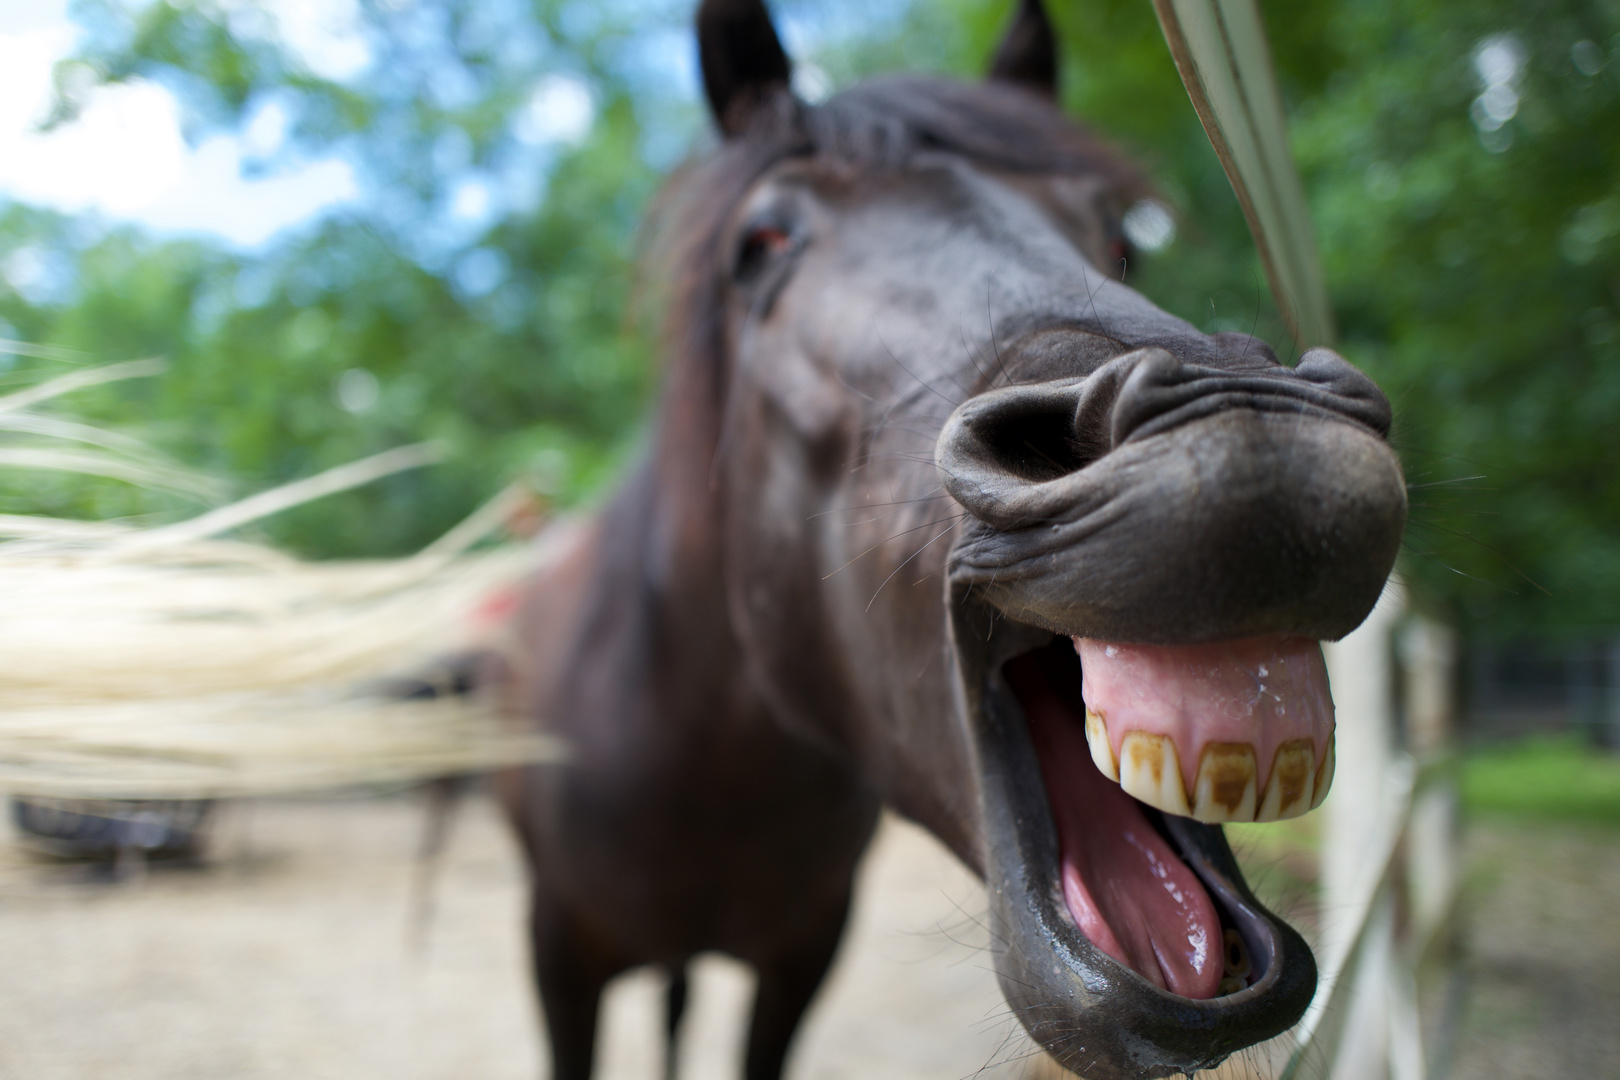
\includegraphics[width=0.7\textwidth]{Schaltskizze.jpg} % Schaltskizze einfügen
    \caption{Schaltskizze des Messaufbaus}
\end{figure}

\subsection{Messergebnisse}
Präsentiere die Messergebnisse, z.B. in Tabellenform oder grafisch. Vergleiche die Messergebnisse mit theoretisch erwarteten Werten und diskutiere etwaige Abweichungen.

\begin{table}[H]
    \centering
    \begin{tabular}{|c|c|c|}
        \hline
        Eingangsspannung & Gemessene Spannung & Abweichung \\
        \hline
        1.00 V & 0.98 V & -0.02 V \\
        2.00 V & 2.01 V & +0.01 V \\
        \hline
    \end{tabular}
    \caption{Messergebnisse des Versuchs}
\end{table}

\subsection{Diskussion}
Diskutiere die Messergebnisse. Was sind die wichtigsten Erkenntnisse? Was lief gut, was könnte verbessert werden?

\section{Fazit}
Ziehe ein Fazit über die Laborversuche. Was wurde gelernt? Welche Herausforderungen gab es? 

\section*{Literaturverzeichnis}
Falls erforderlich, füge hier deine verwendeten Quellen hinzu.

\end{document}
